\section {Method}

\subsection {Mach-Zenhder setup}
This setup for the Mach-Zendher interferometer with phase shifting consists of
a laser (Melles Griot, 05-LHP-111), which is chosen for its long coherens length. 
If we had used white light the components would have to been placed with micrometer 
precision. Using a laser gives a coherens length of about a meter. Though it will 
create noise in the measurements which needs to be weighed in.
The laser beam goes through a beam expander, which due to the nature of lasers having 
a gaussian distribution of intensity, and us wanting a uniform distribution, 
we expand the laser and use only the middle of the beam.
A beam splitter splits the laser beam in two, sending one to a piezo controlled
mirror. 
The piezo is controlled by a computer sending signals to a Nidaq 
(National Instruments, NI USB-6211) which is connected to a high voltage DC OP amp
(burleigh, PZ-70) converting a voltage in a range of -10 V to 10 V 
into 500 V to 1000 V. This gives high precision control of the movement of the 
mirror down to about the order of 10 nm, thus making it possible to move the 
phase of the light wave with great accuracy. From the piezo mirror it is sent 
through a sample cell which contains what we are measuring.
Then it is sent to a beam collector and the interference pattern is picked up by
a CCD camera (Imaging Source, DMK 21BUC03) which is connected to a computer who stores the data.
The second beam travels without hinderance to the collector.

\subsection {Unwrapping}
To analyze the data coming from the camera we used a method called unwrapping.
As we only get an intensity from the camera we have to translate this into something
we can use to analyze the motion of the phase picture. Most of this section
is collected from Optical Measurement of Surface Topography.\cite{omst} 
The interference signal can be expressed as:
\begin {equation}
I(\phi) = I_{DC} + I_{AC}\cos[\theta + \phi]
\end {equation}
where $I_{DC}$ and $I_{AC}$ are fixed coefficients and $\theta$ is the phase and
$\phi$ is the phase shift in terms of the reference mirror displacement.
This equation can then be expanded to
\begin {equation}
I(\phi) = I_{DC} + I_{AC}[\cos(\theta)\cos(\phi) - \sin(\theta)\sin(\phi)]
\end {equation}
Fitting the sine and cosine waves to the interference signal gives the $\sin(\theta)$
and $\cos(\theta)$ terms.
To get the wanted $\theta$ out of this equation it is possible to integrate over
a full cycle of phase $\phi$
\begin {align}
N &= -\int_{-\pi}^{\pi}I(\phi)\sin(\phi)d\phi\\
D &= \int_{-\pi}^{\pi}I(\phi)\cos(\phi)d\phi
\end {align}
Then the phase $\theta$ can be extracted with
\begin {equation}
\tan(\theta) = N/D
\end {equation}
The signal $I(\phi)$ is what we are measuring in the camera and thus by shifting
$\phi$ with evenly placed discrete values $\Delta\phi = \pi/2$ the equation above
becomes
\begin {align}
N &= I_0 +I_1 - I_2 + I_3\\
D &= -I_0 + I_1 + I_2 - I_3
\end {align}
and we get 
\begin {equation}
\tan(\theta) = \frac{I_0 - I_2}{-I_0 + 2I_1 - I_2}
\end {equation}
This can be done for more intensity samples as well, and thus for 7, as we used,
we get
\begin {equation}
\tan(\theta) = \frac{2I_1 - 2I_3}{-I_0 + 2I_2 - I_4}
\end {equation}
By taking the $\arctan$ of this equation we are left with the shifted phase.
But due to the nature of $\tan$, the picture will only have a range of $2\pi$
and therefore have false drops. 
\begin {figure}[ht!]
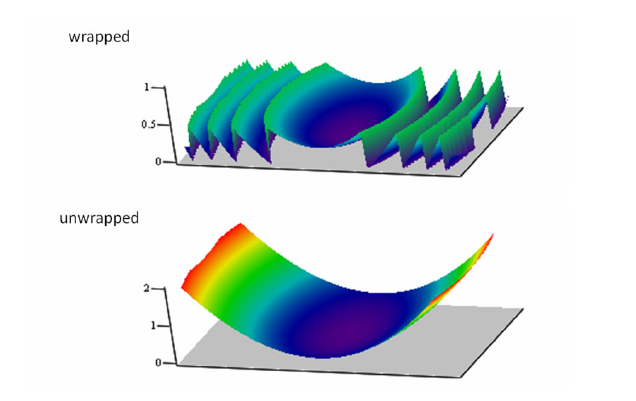
\includegraphics [width=10cm]{bilder/unwrap.png}
\caption {\cite{omst}An illustrative graph of a wrapped and unwrapped phase picture respectivly 
with unit length on the x and y axis, z in radians.}
\end {figure}
To correct these drops we used a 2 dimensional unwrapping algorithm in Matlab called
Constantini phase unwrapping which is based on an article written by M. Constantini 
\cite{const}. This unwrapping of the phase gives a picture of how the phase $\theta$ is moving
as $\phi$ is changed. 

\subsection {Diffusion of table salt in water}
The reason for this experiment was to test the equipment to see if every component
could work together and also get an approximation of how well the accuracy is.
To be able to control the phase shift with the piezo we did a callibration to find
which voltage represented one wavelength. By using the background it was measured to
be a factor of 1.12 which was multiplied to the signal out. Then we placed a rectangle 
sided vial with clear plastic in the middle in front of the beam.

\begin {figure}[ht!]
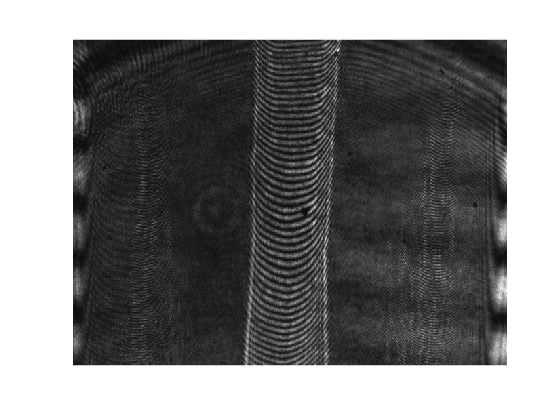
\includegraphics [width=10cm]{bilder/sample.png}
\caption {A vial with nothing in it. The black and white stripes are the inteference %
          of the beam because of the difference in optical path length compared to the %
          unhindered beam. At the far sides there is a background inteference pattern %
          which arise from the camera not being completely aligned.}
\end {figure}

The vial were filled with 2.16 g of water and a piece of 3 mg of salt was added to it.
Now the Matlab program started running which took 
